\chapter{Wire Equivalency Protocol (WEP)}
\label{ch:wep}

\section{Allgemein}
Als erstes, weit verbreitetes Sicherheitsprotokoll hat sich \acrfull{wepLabel} durchgesetzt.
Trotzdem, dass \gls{wepLabel} grosse Schwachstellen und Sicherheitslücken aufweist und diese seit langem (2001) auch bekannt sind, wird \gls{wepLabel} immer noch angewendet (einerseits von alten Geräten, aber auch neue, die aus Kompatibilitätsgründen verschiedene Sicherheitsprotokolle anbieten).

Der Schlüssel ist theoretisch 64 oder 128 Bits lang.
Da davon jedoch 24 Bits für den \gls{ivLabel} verwendet werde, und der unverschlüsselt übermittelt wird, kürzt sich die Schlüssellänge erheblich.
Sprich die effektive Länge des Schlüssel ist 40 oder 104 Bits.
%Die verkürzte Schlüssellänge ist jedoch nicht das Hauptproblem von \gls{wepLabel}.

\section{Angriffe (WEP)}
Nebst fehlerhaften \gls{wepLabel} Implementationen konkreter Hersteller, können allgemeine \gls{wepLabel}-Angriffe in zwei Kategorien eingeteilt werden.\footcite[][126f.]{WrightCache201503}:
In Netzwerke mit aktiven Clients (und entsprechendem Datenverkehr) und solche ohne aktive Clients.

\subsection{Angriff mit einem Opfer Client (WEP)}
Der Angriff auf ein Netzwerk mit Clients ist einfacher, kann jedoch mehr Geduld beanspruchen.

Ein durchgeführtes Beispiel ist im \secref{sec:wepAttack} dokumentiert.





\subsection{Angriff ohne einem Opfer Client (WEP)}
\todo{Angriff ohne Opfer Client kurz erläutern}

\section{Konkreter Angriff}
\label{sec:wepAttack}
\todo{Einleitungstext}

\subsection{Setup}
\subsubsection{Hardware}
Nebst der in \secref{sec:testEnvroiment} beschriebene Hardware wurde ein ältere Swisscom Router \textit{Netopia  3357NWG}\footcite{Netopia_3347_57nwg_de_2015-04-06} verwendet. Der Router wurde mit einem 10-stelligen hexadezimalen Passwort eingerichtet.

\subsubsection{Software}
OS X stellt, innerhalb von Xcode\footcite{Xcode_Apple_Developer_2015-04-06}, bereits nützliche Wireless Analyse Tools zur Verfügung.
Zudem kann via \textit{Homebrew}\footcite{Homebrew__The_missing_package_manager_for_OS_X_2015-04-06} die \textit{aircrack-ng}\footcite{Aircrack-ng_2015-04-06} Programm Sammlung installiert werden.

\begin{framed}
	\textbf{Bemerkung:} Obwohl das \textit{KisMac2}\footcite{IGR_Software_KisMac2_2015-04-06} viel erwähnt wird, hat sich dieses Programm während dieser Arbeit nicht bewährt. Es stürzte vermehrt ab. Darum die Empfehlung mit dem von Xcode bereitgestellten "`airport"' Konsolen-Programm zu arbeiten.
\end{framed}

\subsection{Ausführung}
Mit dem "`Wireless Diagnostics"' Tool von Apple kann via \textit{Window} $\rightarrow$ das \textit{Scan} und das \textit{Sniffer} Programm geöffnet werden.
Mit dem \textit{Scan} Programm können verfügbare Netze und deren Channels gefunden werden.

\begin{figure}[H]
	\centering
	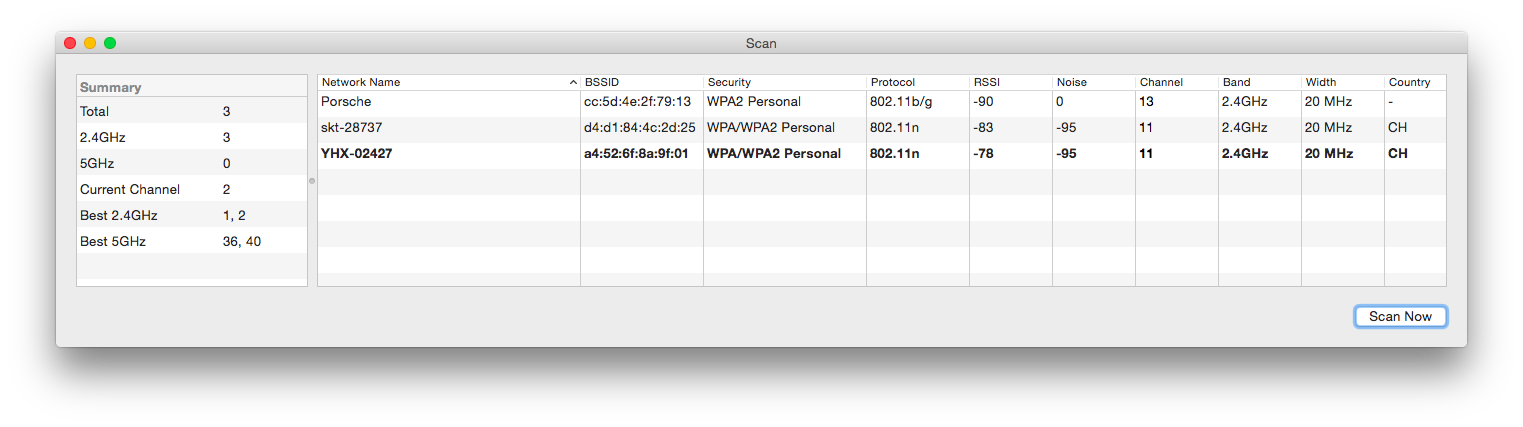
\includegraphics[width=1.0\textwidth]{images/wep/scan.png}
	\caption{Scanner -- OS X Wireless Diagnostics}
\end{figure}

Mit dem \textit{Sniffer} können benötigte Daten aus einem konkreten Netz aufgezeichnet werden. Es werden ca. 5'000 \gls{ivLabel}'s benötigt um den Schlüssel zu berechnen. Eine solche Aufzeichnung (capture) dauert unterschiedlich lange, je nach Nutzung des Netzes. Wird das Netz viel gebraucht, geht es schneller.

\begin{figure}[H]
	\centering
	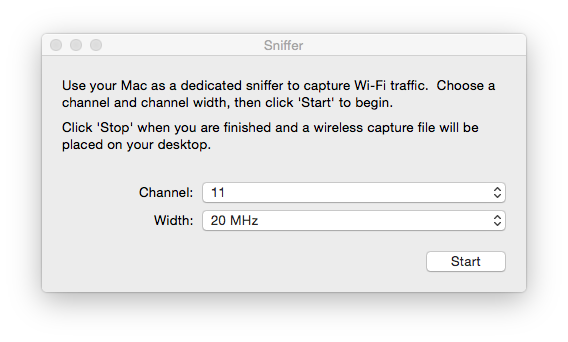
\includegraphics[width=0.8\textwidth]{images/wep/sniffer.png}
	\caption{Sniffer -- OS X Wireless Diagnostics}
\end{figure}

%\begin{wrapfigure}{r}{0.6\textwidth}
%	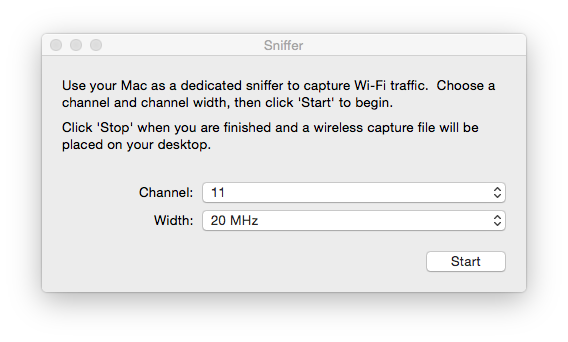
\includegraphics[width=1.0\linewidth]{images/wep/sniffer.png}
%	\caption{OS X Wireless Diagnostics: Sniffer}
%\end{wrapfigure}

Der Sniffer kann auch direkt über die Kommandozeile ausgeführt werden:
\begin{lstlisting}[style=lstStyleFramed]
sudo ln -s /System/Library/PrivateFrameworks/Apple80211.framework/Versions/Current/Resources/airport /usr/sbin/airport
sudo airport en0 sniff <CHANNEL>
\end{lstlisting}

Anschliessend können die Daten, vom \textit{Sniffer} mit dem \textit{aircrack-ng} ausgewertet werden:
\begin{lstlisting}[style=lstStyleFramed]
aircrack-ng -b 00:0f:cc:b0:1a:c8 /private/tmp/airportSniff*.cap
\end{lstlisting}

So wird einem, falls genügend \gls{ivLabel}'s vorhanden sind, der \gls{wepLabel} ausgegeben (Dauer: 2 Sek.).
\begin{figure}[H]
	\centering
	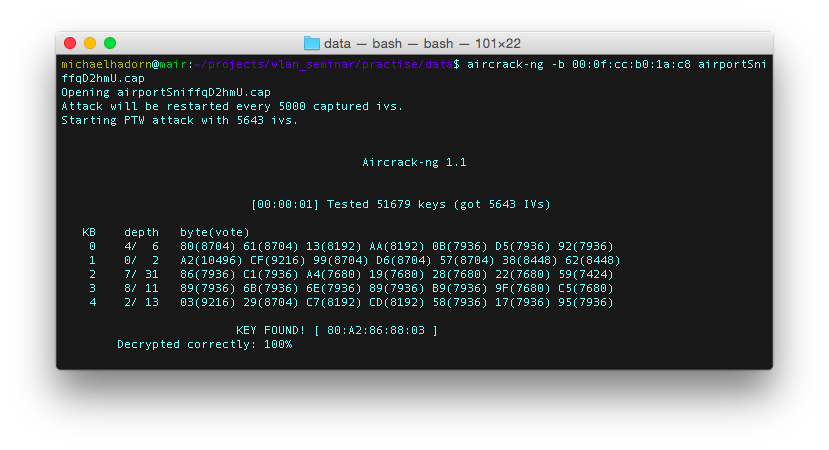
\includegraphics[width=1.0\textwidth]{images/wep/aircrack-ng.png}
	\caption{aircrack-ng -- Terminalausgabe}
\end{figure}
